% Written by src/detection/final_figures.py; needs \usepackage{graphicx} and results/figures/ in \graphicspath.
\begin{figure*}[tb]
  \centering
  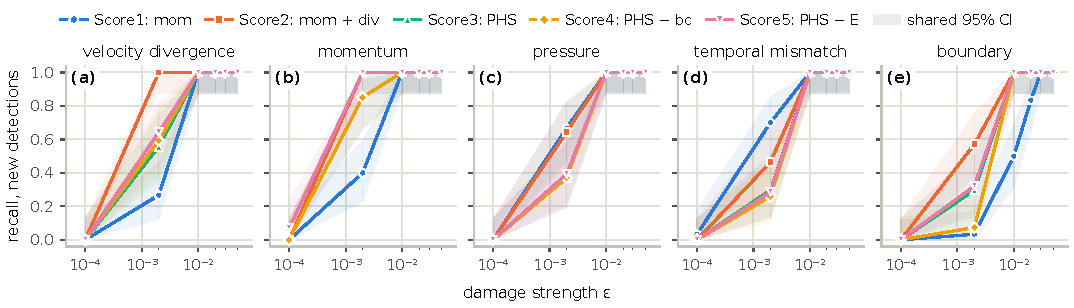
\includegraphics[width=\textwidth]{fig_recall_vs_eps_new_detections.pdf}
  \caption{Recall as in Fig.~\ref{fig:recall_vs_eps}, but only over the cases whose clean field the score does not flag, since flagging a damaged field of an already-flagged case is no new detection. Cases per score: Score1 30, Score2 28, Score3 27, Score4 27, Score5 28; bands: exact 95\% confidence intervals. At $\varepsilon = 0.0001$ the only new detections are cases whose clean score is just below $\tau$: Score1, temporal mismatch damage: case 34 (clean score 0.98 times $\tau$); Score5, momentum damage: case 31 and case 45 (clean score 0.99 and 0.99 times $\tau$). Every score flags every damaged field from $\varepsilon = 0.01$ on (already from 0.002 for Score2 with velocity divergence and momentum damage and Score5 with momentum damage), except Score1 for boundary damage (15/30 at 0.01 and 25/30 at 0.02).}
  \label{fig:recall_vs_eps_new_detections}
\end{figure*}
